\documentclass[14pt,fleqn]{extarticle}
\RequirePackage{prepwell}
\previewoff
\begin{document}

\newcommand\ysq{32-x^2}
\newcommand\ycirc{\sqrt{\ysq}} 
\newcommand\intga{\int_0^4}
\newcommand\intgb{\int_4^{\sqrt{32}}}

Using integration, find the area of the region in the first quadrant 
enclosed by the $x-$axis, the line $y=x$ and the circle $x^2+y^2 = 32$

\newcard

Only the shaded region satisfies the two conditions

\begin{itemize}
\item{Is in the first quadrant} 
\item{Is enclosed by the circle, the line $y=x$ and the $x-$axis} 
\end{itemize} 

\begin{center}
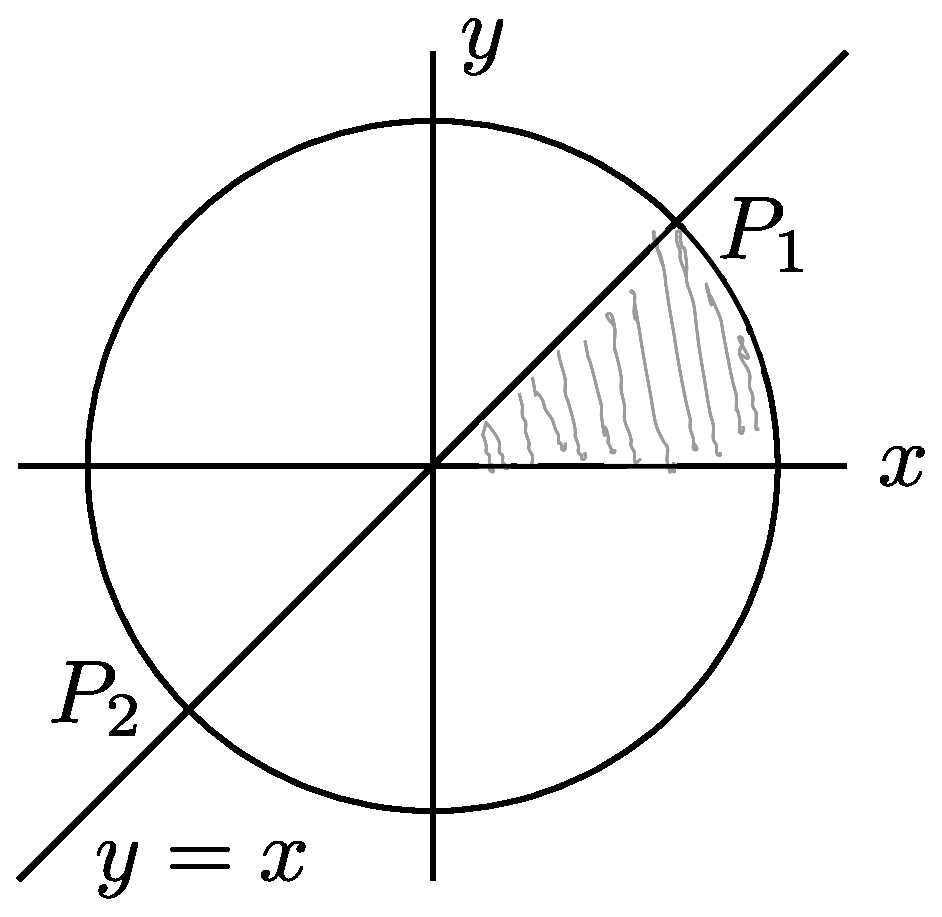
\includegraphics[scale=0.3]{figure.eps}
\end{center}

\newcard

The line and the circle will intersect at $P_1 = (4,4)$ in the first quadrant 
        
\newcard 

The line and the circle will intersect at $P_1 = (3,3)$ in the first quadrant 

\newcard 

The line and the circle will intersect when 

\begin{align}
	y = x = \ycirc &\text{ or } x^2 = \ysq \\
	\text{or } 2x^2 = 32 &\implies x = \pm 4 
\end{align}

This gives us two points -- $P_1 = (4,4)$ and $P_2 = (-4,-4)$ \newline 

But only $P_1$ lies in the first quadrant. Hence, that is the point we are interested in 

\newcard 

The required area $R$ is therefore 
\[ \quad R = \underbrace{\intga x\cdot dx}_P + \underbrace{\intgb \ycirc\cdot dx}_Q \]

\newcard 

As you can see from the figure in the previous step, the required area is composed of two parts 

\begin{center}
  \begin{tabular}{NcN}
   \toprule
        \text{Label} & Area under & \text{Integral} \\
   \midrule 
   P & Line & \intga x\cdot dx \\
    \midrule 
    Q & Circle & \intgb \ycirc\cdot dx \\
    \bottomrule
  \end{tabular}
\end{center}

Hence $R = \intga x\cdot dx + \intgb \ycirc\cdot dx$ 

\newcard 

\begin{center}
  \begin{tabular}{NcNN}
   \toprule
        \text{Label} & Area under & \text{Integral} & \text{Value}\\
   \midrule 
   P & Line & \intga x\cdot dx & 8 \\
    \midrule 
    Q & Circle & \intgb \ycirc\cdot dx & 4\pi-8\\
    \bottomrule
  \end{tabular}
\end{center}

Therefore, $R = P+Q = 4\pi\text{ sq. units}$ 

\begin{align}
P &= \intga x\cdot dx = \left[\frac{x^2}{2} \right]_0^4 = \left[\frac{16}{2}-0 \right] = 8\\
Q &= \intgb\ycirc\cdot dx \\
&= \underbrace{\left[\frac{x}{2}\ycirc + 16\cdot \sin^{-1} \frac{x}{\sqrt{32}} \right]_4^{\sqrt{32}}}_{\int \sqrt{a^2-x^2}\cdot dx = \frac{x}{2}\sqrt{a^2-x^2} + \frac{a^2}{2}\sin^{-1} \frac{x}{a}} \\
&= \underbrace{\left(16\cdot \frac{\pi}{2}\right)}_{x = \sqrt{32}} - \underbrace{\left(\frac{4}{2}\sqrt{16} + 16\sin^{-1} \frac{4}{\sqrt{32}} \right)}_{x=4} \\
&= 8\pi - \left(8 + 16\cdot \sin^{-1}\frac{1}{\sqrt{2}} \right) \\
&= 8\pi - \left(8 + 16\cdot \frac{\pi}{4} \right) = 4\pi - 8 \\
\therefore R &= P + Q = 8 + \left(4\pi-8 \right) = 4\pi
\end{align}
\end{document}